\chapter{Optimal Experiment Design}
\label{sec:OptimalDesign}

In the following chapter, a simple experiment is designed with the main objective of optimizing glucose data identifiability, regardless of the model used. Several safety measures have to be accounted for, including risk to hypo and hyperglycemia to the patient. The experiments are desired to be home-made, performed entirely by the patient, with few to non influence into the daily life of the patient.

\section{Introduction}
\label{sec:Introductionoptext}

Optimal experiment design requires of the designer to determine the experimental parameters to be used for optimization of identifiability. The diabetic patient model inputs are the variables that can be adjusted for the adequation of the experiment. For obtaining an optimal experiment, the best combination of the inputs regarding at the identifiability of the model is to be found.

Another variable usually considered in the optimization of the inputs is the sampling period of the measurements. In the experiments to be performed in this thesis, the measurements are considered to be sampled by a CGM, so the measurements are taken with the sampling period of the monitor (every 5 minutes), and the number of samples linearly increases with the experiment's length. The design problem is then transformed into how long the experiment should last. Usually, identifiability of the model increases with the number of samples because the experiment's data get richer, so the boundary of the experiment time is not of identifiability issues but of safety reasons. After medical consultation and examination of the resources for the experiments, it was decided that the length of the experiment was to be fixed at five hours after a meal, considering that most of the postprandial response and input excitation occurs in this period.

The most common inputs of a complete glucoregulatory model are two, the meals and the insulin infusion (supposing insulin pump treatment). Meals are usually considered as a disturbance, but in this work, mathematical models are used for simulating the meal absorption as an input to be designed. Insulin postprandial infusion is considered as an input as well. Both inputs can be parametrized as:
\begin{itemize}
	\item Parametrization of the meal system input:
\begin{enumerate}
	\item Meal size
	\item Meal composition
\end{enumerate}
	\item Parametrization of the insulin system input:
\begin{enumerate}
	\item Insulin bolus size
	\item Insulin bolus time (relative to meal time)
	\item Basal infusion rate
\end{enumerate}
\end{itemize}
Regarding meal composition, the published parameters in literature for the meal model analyzed in here, the UVA gastrointestinal model, were identified under the specific conditions listed below:
\begin{itemize}
	\item Caloric input: 10 kcal/kg
	\item Carbohydrate: 45\%
	\item Protein: 15\%
	\item Fat: 40\%
	\item Carbohydrate estimation and uncertainty: 90 $\pm$ 5 g
\end{itemize}
Carbohydrate estimation represents the size of the meal. The rest of the parameters determine the gastric emptying profile, and the identification performed in \cite{man2006system} produced the parameter values shown in Table \ref{tab:dallaman} based on the specified meal composition. Unfortunately, no identifications on different meal compositions have been performed on this model. Therefore, if optimum performance of the model is desired, experiments with this model are to be performed with similar composition to that shown in \cite{man2006system}. The size of the meal is  one of the parameters for the experiment design.

Regarding at the insulin input, the parameters chosen for optimization of the experiment design are much more complex than the those of the meal ingestion, which is only considered as an impulse. The insulin pump treatment can have any shape imaginable in accordance to the pump limitations. Designing an absolutely free insulin profile, i.e. a non-parametric input, would be too expensive in computational terms (for more information see \cite{walter1997}), so a parametric input is chosen. The classic profile of basal-bolus infusion is preserved in this experiment design for simplification purposes and to increase the patient's compliance with the experiment.

Once decided that a traditional treatment is going to be followed, the only parameters to be chosen for the experiment design are the amount of insulin to be given as a bolus, the basal insulin level, and the instant the bolus is administered. The basal rate was discarded from the parameter optimization set after a pilot experiment design. In this first experiment, the influence of basal was found to be neglectible on the model's identifiability when compared with the rest of parameters (meal and bolus). Also, adding a variable basal rate for each patient increased the number of optimization parameters too much, making the optimization much computationally intensive, which was not desired.

In summary, the experiment conditions to be tuned in the optimization are:
\begin{itemize}
\item $\tau$ - Delay of the insulin bolus with respect the meal time, in minutes. A positive delay means that the insulin dose is given after the meal and viceversa. The boundaries for the optimization problem are set to -60 and 300 minutes. Maximum advancement of the insulin bolus is defined so as to prevent hypoglycemic events.
\item Meal - The size of the meal in grams of carbohydrates. The boundaries for the optimization problem are 0 and 100 grams of carbohydrates.
\item Bolus - The amount of bolus insulin units to be given. The boundaries for the optimization problem are 0 and 10 insulin units. These boundaries were chosen using an insulin-to-carbohydrate ratio of 1:10 as population mean.
\end{itemize}
Only one meal per day is considered in order to avoid influences from the circadian variation of insulin sensitivity. The vector $\Xi$ (as seen in equation \eqref{eq:index}) is a vector of size $3\cdot n_d$, where $n_d$ is the number of days of monitoring. This vector is the output of the experiment design.

Given that the problem is highly non-linear (due to non-linearities of the index and the model) SSM global optimizer was used to obtain the solutions, as introduced in the Section \ref{sec:ScatterSearchForMatlab}. The constraints for the optimization problem are the restrictions of the blood glucose in order to keep the patient under safe health conditions. The simulation was forced to start from equilibrium in a blood glucose level of 100 mg/dL. The maximum level of glucose (hyperglycemic bound) was set to 250 mg/dL and the minimum level (hypoglycemic bound) was set to 70 mg/dL. These boundaries are respected at all times during the optimization of the experiment design.

Before the actual experiment design, a selection of the most relevant parameters is performed. A very simple analysis of identifiability is carried out on each of the models tested in order to discard non-relevant parameters that may induce optimality problems in the minimization of the experiment design. Repeated iterations of sensitivity analysis are done over the full model parameter set, iteratively removing any parameter that produces either singularity of the FIM or that presents a coefficient of variation larger that 30\%.

In the following lines results for experiment design in diabetes for two different models are shown. Despite the fact that Bergman's model has been proven unreliable for simulating some glucose dynamics, it is desirable to execute the experiment design methodology varying the models used in order to make the experiments as model-independent as possible. Therefore the first experiment design presented is calculated for this model. After that, experiments designed for the modified Panunzi model are displayed. Qualitative information can be extracted from every model's designed experiment. Common conclusions will be synthesized after the experiment design with both models considered and a feasible, patient-friendly protocol will be developed

\section{Experiments designed with Bergman's model}
\label{sec:ExperimentsDesignedWithBergmanSModel}

Initially, Bergman's endogenous model requires for the identification of three parameters, but two more are to be identified in a realistic identification experiment: distribution volume and basal glucose. Glucose distribution volume affects the glucose concentration with respect to the glucose inputs of the system throughout the postprandial period, and basal glucose states for the initial state of the glucose simulation, which for Bergman's model (equation \eqref{eq:Bergman3}) also affects the dynamics of the system. To complete the simulation of a diabetic patient, UVA's gastrointestinal model is implemented along with Cambridge's insulin absorption model. UVA's gastrointestinal model is one of the few models presented in literature with identification on mixed meals instead of glucose solution (even though the mixed meal used is far from being a classic meal), and that is the reason to choose it for the virtual patient's simulation. The Cambridge insulin absorption model was chosen based on the analysis of Willinska \textit{et al.} where it was compared against 11 literature models \cite{wilinska2005insulin} and showed excellent prediction capabilities. Bergman's endogenous model combined with UVA's glucose absorption model and Cambridge's insulin subcutaneous model sums up a total of 17 parameters, described in Table \ref{tab:bergmanparameters}.

%\begin{figure}[hbtp]
%\centering
%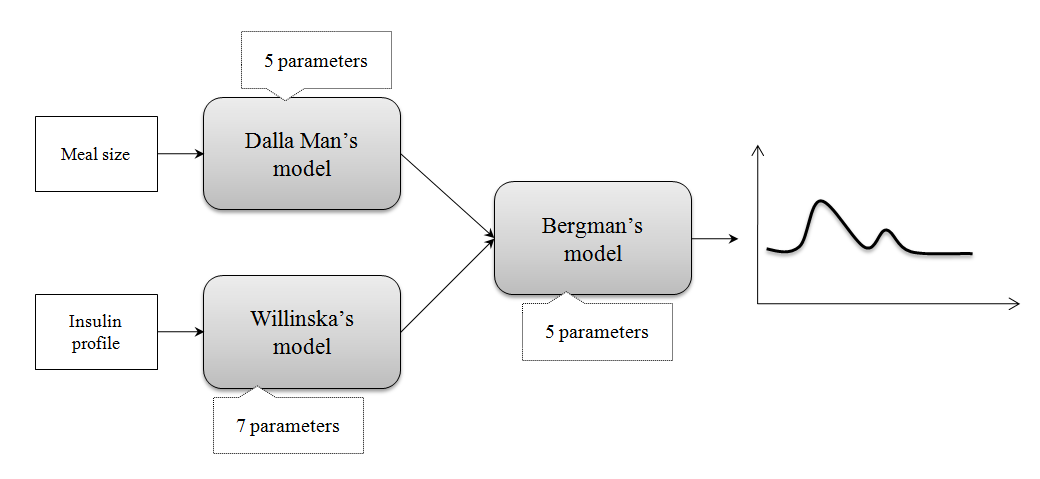
\epsfig{file=Figures/bergmanparameters.png, width=0.8\textwidth}\caption{Total number of parameters to be identified in Bergman's model}
%\label{fig:bergmanparameters}
%\end{figure}

\begin{table}[hbtp]
	\centering
	\begin{tabular}{| c | c | c | c |}
	\hline 
	Model	& Number & Parameter & Meaning \\
	\hline 
	Endogenous & 1 & $p_{1}$ & Glucose efficiency \\
	 & 2 & $p_{2}$ & Insulin action rate of disappearance\\
	 & 3 & $p_{3}$ & Insulin action rate of appearance \\
	 & 4 & $Vol_{g}$ & Distribution volume of glucose \\
	 & 5 & $G_{b}$ & Basal glucose \\
	\hline
	Gastric & 6 & $K_{abs}$ & Glucose absorption rate in the gut \\
	 & 7 & $K_{max}$ & Maximum gastric emptying \\
	 & 8 & $K_{min}$ & Minimum gastric emptying \\
	 & 9 & $b$ & Involved in the gastric emptying \\
	 & 10 & $c$ & Involved in the gastric emptying \\
	\hline
	Insulin & 11 & $V_{i}$ & Distribution volume of insulin \\
	 & 12 & $k$ & Proportion of insulin in the slow channel\\
	 & 13 & $k_{a1}$ & Transfer rate in the slow channel \\
	 & 14 & $k_{a2}$ & Transfer rate in the fast channel \\
	 & 15 & $k_{e}$ & Insulin elimination \\
	 & 16 & $V_{MAX,LD}$ & Michaelis-Menten parameter \\
	 & 17 & $k_{M,LD}$ & Michaelis-Menten parameter \\
	\hline
	\end{tabular}
\caption{Parameters integrated in Bergman's model.}
\label{tab:bergmanparameters}
\end{table}

Considering only blood glucose as the measurable output of the system, identifiability of all parameters is not expected. A three days experiment as the identification period was assumed. Later in this chapter, the choice of a three days experiment is discussed and proven to be adequate for the type of experiments being designed. A sensitivity analysis previous to the experiment design was performed, and the results are shown in Table \ref{tab:bergmanCV}. Only three iterations were needed to obtain a feasible set of parameters for identification on the Bergman model, but the algorithm initially discarded 8 parameters due to non-invertability of the FIM, which is closely related to structural non-identifiability. Indeed, the structural combination of Bergman model with the selected input models rendered many parameters difficult to identify just from glucose concentration data. Should richer data be available, such as plasma insulin data or tracer data of glucose flux from the gut, the sensitivity analysis would change.

\begin{table}[hbtp]
	\centering
	\begin{tabular}{ c | c | c | c | c }
	\multirow{2}{*}{Number} & \multirow{2}{*}{Parameter} & \multicolumn{3}{c}{Iteration} \\
	& & 1 & 2 & 3 \\
	\hline 
	1 & $p_{1}$ & - &	- &	- \\
	2 & $p_{2}$ & - &	- &	-\\
	3 & $p_{3}$ & - &	-	& - \\
	4 & $Vol_{g}$ & 0.25 & 0.14 & 0.13 \\
	5 & $G_{b}$ & 0.12 & 0.08 & 0.07 \\
	6 & $K_{abs}$ & - & - & - \\
	7 & $K_{max}$ & 0.25 & 0.24 & 0.23 \\
	8 & $K_{min}$ & 0.42 & - & - \\
	9 & $b$ & 0.16 & 0.12 & 0.04 \\
	10 & $c$ & 0.20 & 0.18 & 0.09 \\
	11 & $V_{i}$ & - & - & - \\
	12 & $k$ & 0.34 & 0.33 & - \\
  13 & $k_{a1}$ & 0.31 & 0.22 & 0.09 \\
	14 & $k_{a2}$ & - & - & - \\
	15 & $k_{e}$ & 0.22 & 0.14 & 0.12 \\
	16 & $V_{MAX,LD}$ & - & - & - \\
	17 & $k_{M,LD}$ & - & - & - \\
	\end{tabular}
\caption{Bergman's model parameter coefficient of variation (CV) for a three meals simulation. Each column represents an iteration in the sensitivity analysis. Parameters fixed to nominal values due to non-identifiability are indicated by a dash. Parameters fixed at iteration 1 are cause of structural non-identifiability.}
\label{tab:bergmanCV}
\end{table}

The final number of parameters identifiable, out of the initial 17, is 7. Only two of those parameters are part of the endogenous model, while three characterize the gastrointestinal model, and the other two are part of the insulin model, as can be seen in Figure \ref{fig:bergmanparametersidentifiable}.

\begin{figure}[hbtp]
\centering
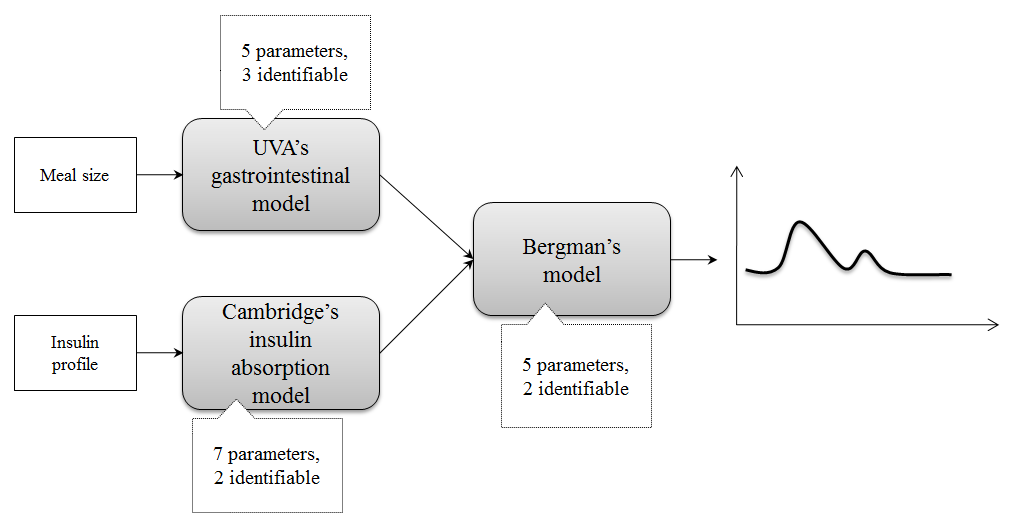
\epsfig{file=Figures/bergmanparametersidentifiable.png, width=\textwidth}\caption{Optimal set of parameters for Bergman's model combined with UVA's gastrointestinal model and Cambridge insulin absorption.}
\label{fig:bergmanparametersidentifiable}
\end{figure}

Those 7 parameters are used to optimally express the identifiability of the model. The experiments designed next expres the model's identifiability in the optimization index by using this optimal set of parameters. The range of days considered for experimentation is from one to four days. At the end of the experiment design for all the models under study, the best option was chosen from within of all the experiments designed, including the different options of parameter sets, models, and length of the experiments.

In the next lines, experiments designed comprising one, two, three and four days of monitoring are displayed. All experiments are designed using D-optimality, as described in Section \ref{sec:Optimizationofidentifiability}.

\begin{itemize}
\item{The results of an experiment designed for \textit{one} day of monitoring consisting on the five following hours to a meal are: $\tau = -31.59$ minutes, Meal $= 100$ g CHO and Bolus $=10$ IU. %is shown in Table \ref{tab:bergmanexperiment1day}.
%\begin{table}[hbtp]
%  \begin{center}
%	\begin{tabular}{| c | c | c |}
%	\hline 
%	Experiment & Units & Day 1 \\
%	\hline 
%	$\tau$ & minutes & -31,59 \\
%	Meal & gr CHO & 100 \\
%	Bolus & IU	& 10 \\
%	\hline	
%	\end{tabular}
%  \end{center}
%  \caption{Experiment conditions for the Bergman's model design considering one day of monitoring}
%	\label{tab:bergmanexperiment1day}
%\end{table}
In the case of only being able of monitoring one day, the optimum experiment to be followed requires the diabetic patient to advance the bolus approximately half hour, and then eat a large meal (100 grams CHO). It is worth remembering that 100 grams of carbohydrates is the top value given to the optimizer for the experiment design. Also, 10 is the top boundary for the bolus variable in the optimization, and it is the corresponding value of insulin for an standard treatment of insulin boluses for a 100 grams of carbohydrates meal. This means that, in addition to maximizing identifiability of the model, the experiment design keeps the patient under standard glycaemic control. This is a direct response to the output restrictions to the simulation model that force the patient's glucose to be within healthy range. The glucose profile associated to the experiment described can be seen in Figure \ref{fig:bergmanexperiment1day}.

\begin{figure}[hbtp]
\centering
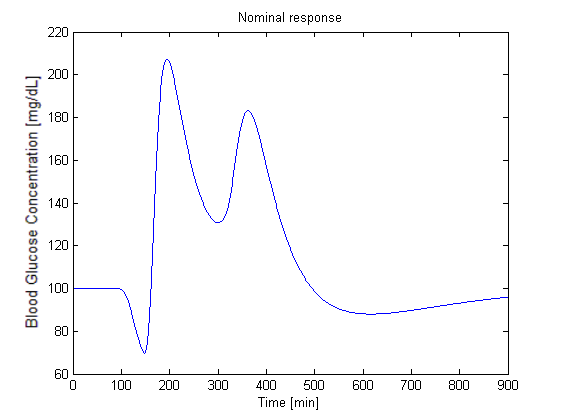
\epsfig{file=Figures/Berman_experiment_1day.png, width=0.9\textwidth}\caption{Bergman's model response to the proposed experiment for 1 day. Meal is ingested at time 120 min.}
\label{fig:bergmanexperiment1day}
\end{figure}

The glucose profile shows a very quick response to the advanced insulin bolus, dropping quickly to a level of approximately 70 mg/dL. This level is the safety threshold indicated as a constraint to the output in the optimization algorithm in order to keep the patient under safe conditions. This simulation shows how the optimizer is exciting the output variable as much as possible, and always keeping the (virtual) person safe.}

\item{The conditions of the experiment designed for \textit{two} days monitoring are:

\begin{itemize}
	\item Day 1. $\tau = 25.23$ minutes, Meal $= 86.81$ g CHO and Bolus $=10$ Insulin Units
	\item Day 2. $\tau = -29.58$ minutes, Meal $= 100$ g CHO and Bolus $=10$ Insulin Units
\end{itemize}

In this new experiment two different therapies are applied to the patient. The second day is a replicate of the conditions of the experiment design corresponding to only one day. In the first day of identification, a bolus of 10 insulin units is delayed approximately 25 minutes, for a meal of 86.81 grams of carbohydrates. In this case the proportion of insulin units to grams of carbohydrates of the meal is not maintained, thus, not a standard glycaemic control is performed on the patient (including the effect of the delay). The glucose profile for the designed two-day experiment is shown in Figure \ref{fig:bergmanexperiment2day}.

\begin{figure}[hbtp]
\centering
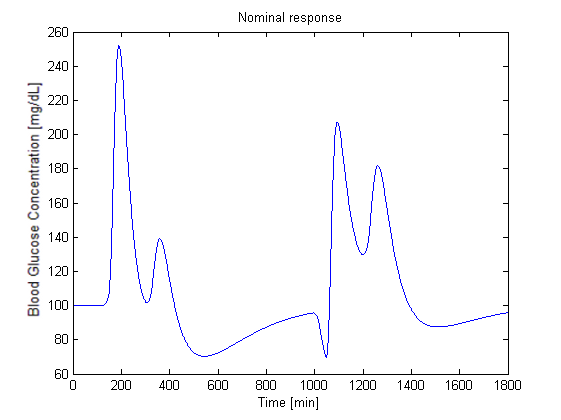
\epsfig{file=Figures/Berman_experiment_2day.png, width=0.9\textwidth}\caption{Bergman's model response to the proposed experiment for 2 days. Meals are ingested at time 120 and 1020 min.}
\label{fig:bergmanexperiment2day}
\end{figure}

Observing the first day response of the model to the proposed experiment, the fact of non-proportionality of insulin to carbohydrates makes more sense. The model moves from 250 mg/dL down to 70 mg/dL, which are the top and bottom safety thresholds in the experiment design optimization algorithm. The optimizer is exciting the measurable variable (blood glucose) through all the feasibility glucose range in order to maximize identifiability. Given that in the first day, due to the delay of the insulin bolus, there is no falling of the blood glucose to the lowest level, it has to drop to that level after the meal, that is why the insulin bolus is still relatively big with respect to the size of the meal. Given those values, the maximum amount of carbohydrates for that meal, so that the experiment does not exceed the upper safety threshold, is $86.81$.

It is interesting to understand why the two days differ in the relative bolus administration time. In the first day, no insulin excitation is applied in approximately 30 minutes from meal time and all the information extracted from that period is contributing to increase the identifiability of the gastrointestinal input model, the UVA model. In the other day, the opposite situation is happening: only the insulin subcutaneous model is experimenting excitation in the first period of the simulation, so information from glucose is affecting only the parameters of that model. The strongest the variation of the states of the model in that period, the greater the identifiability will be.}

\item{The conditions of the experiment designed for \textit{three} days monitoring are:
\begin{itemize}
	\item Day 1. $\tau = 26.43$ minutes, Meal $= 85.6$ g CHO and Bolus $=10$ Insulin Units
	\item Day 2. $\tau = -30.44$ minutes, Meal $= 100$ g CHO and Bolus $=10$ Insulin Units
	\item Day 3. $\tau = -30.71$ minutes, Meal $= 100$ g CHO and Bolus $=10$ Insulin Units
\end{itemize}

In this case, the advancing of the bolus is repeated two days. Given that the meals do not have to be consecutive, or that one day does not have any relation to the others, the order of the experiment days is not relevant for the result of the experiment. The glucose profile for the designed three-day experiment is shown in Figure \ref{fig:bergmanexperiment3day}.

\begin{figure}[hbt]
\centering
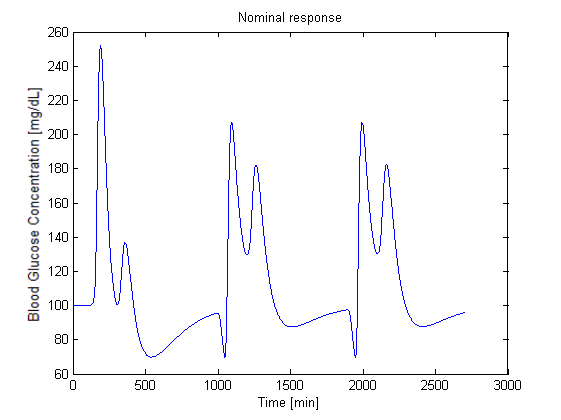
\epsfig{file=Figures/Berman_experiment_3day.png, width=0.9\textwidth}\caption{Bergman's model response to the proposed experiment for 3 days. Meals are ingested at time 120, 1020 and 1920 min.}
\label{fig:bergmanexperiment3day}
\end{figure}

The second and third days are virtually the same experiment, and the first day displays again the extreme excitation of glucose between safety boundaries. It can be appreciated once again how there is a separation of dynamics between the different input models.}

\item{The conditions of the experiment designed for \textit{four} days monitoring are:
\begin{itemize}
	\item Day 1. $\tau = 25.44$ minutes, Meal $= 86.81$ g CHO and Bolus $=10$ Insulin Units
	\item Day 2. $\tau = 14.36$ minutes, Meal $= 99.64$ g CHO and Bolus $=10$ Insulin Units
	\item Day 3. $\tau = -29.92$ minutes, Meal $= 100$ g CHO and Bolus $=10$ Insulin Units
	\item Day 4. $\tau = -30.88$ minutes, Meal $= 100$ g CHO and Bolus $=10$ Insulin Units
\end{itemize}

In this final case the two last days are repeated again, displaying an advance of the insulin bolus, and a new delayed bolus profile appears, but in this case with a big meal. The delay on the bolus is smaller so that the meal can be bigger, contributing to the improvement of identifiability of UVA's gastrointestinal model. The glucose profile for the designed four-days experiment is shown in Figure \ref{fig:bergmanexperiment4day}.

\begin{figure}[hbt]
\centering
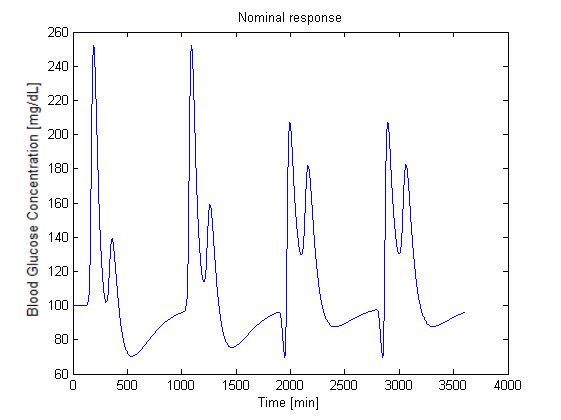
\epsfig{file=Figures/Berman_experiment_4day.png, width=0.9\textwidth}\caption{Bergman's model response to the proposed experiment for 4 days. Meals are ingested at time 120, 1020, 1920 and 2820 min.}
\label{fig:bergmanexperiment4day}
\end{figure}

As it can be observed, there is not much difference in the first two days of identification because the difference in the meal size is relatively small.}
\end{itemize}

The most relevant observation of this experiment design with the Bergman model is that separating dynamics of the input models is the key to improve the identification of the whole system. It is better for a model general identifiability to advance the bolus rather than having it delayed following the cases of one day experiment design (advancing bolus) and three-day experiment design (advancing bolus two days out of three). However, a better scenario comprises both situations, advancing and delaying the bolus. A minimum of a two-day experiment is then required for basic identification of the system. 

Experiment's length is selected attending to: 1) identifiability conditions, 2) experiment parameters and 3) practical implementation aspects. It has been stated that a minimum of two days for monitoring seems reasonable for identification purposes due to the two different profiles of experiment. Naturally, as more data (more days of experiment) is available, the probability of a satisfactory identification increases. However, the practical implementation aspect limits the number of days in a experiment. In Figure \ref{fig:Bergmandays} evolution of identifiability of each parameter of the optimal set in Bergman's model can be observed for all the cases exposed before and after the experiment design.

\begin{figure}[hbtp]
\centering
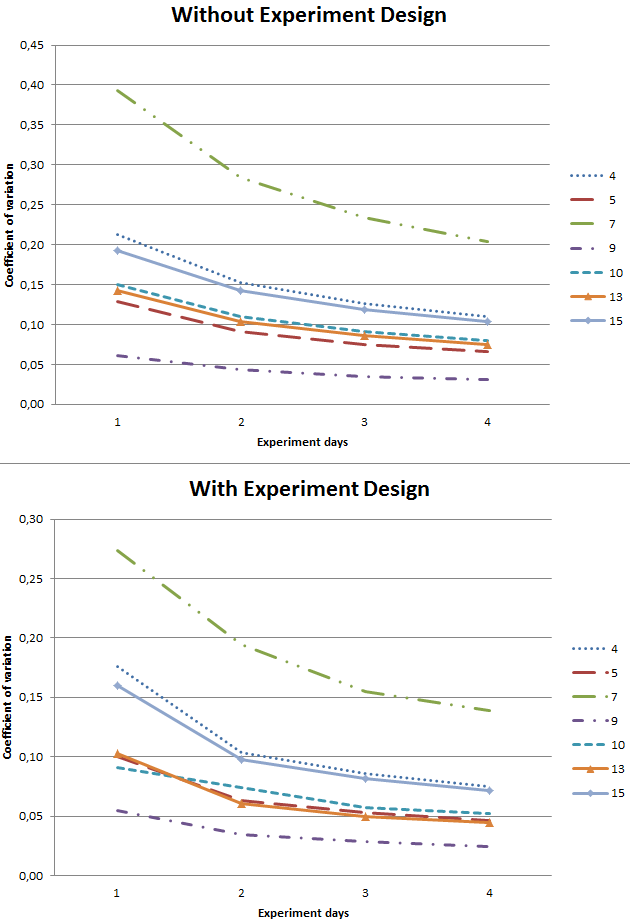
\epsfig{file=Figures/Bergmandays.png, width=0.8\textwidth}\caption{Coefficient of variation for Bergman's model's parameters. Top graph shows the evolution of the parameters' identifiability with experiment length. Bottom panel displays the identifiability of the same parameters applying the designed experiments. It is clearly shown how identifiability increases (CVs decrease) with experiment length. Parameter numeration is equivalent to that of Table \ref{tab:bergmanCV}.}
\label{fig:Bergmandays}
\end{figure}

An abrupt decrease in the coefficient of variation of all parameters occurs between one and two days of monitoring, reinforcing the mentioned minimum of identifiability in two days, both for the experiments with and without optimal design. If more days are added to the experiment identifiability keeps increasing less rapidly. Very similar trends in the identifiability rise are observed for both the original experiments and for the optimal designed experiments. The identifiability levels, as measured by coefficient of variation of the parameters are much lower for any experiment length when choosing the optimal design for the experiment. A three-day experiment was chosen thinking on the limitations introduced by the clinical implementation of the experiment. It is desired to have as many identification days as validation days, which makes the real monitoring period twice as long as the experiment designed. Given that the average sensor lifetime in a continuous glucose monitor is approximately one week, the three days experiment was chosen as monitoring duration, for maximization of identifiability. Results have to be compared with designed experiments based on other models in order to make the experiments as model-independent as possible. Comparison between the coefficients of variation of a three-day identification experiment is displayed in Figure \ref{fig:Bergmanoptdesign3days}.

\begin{figure}[hbt]
\centering
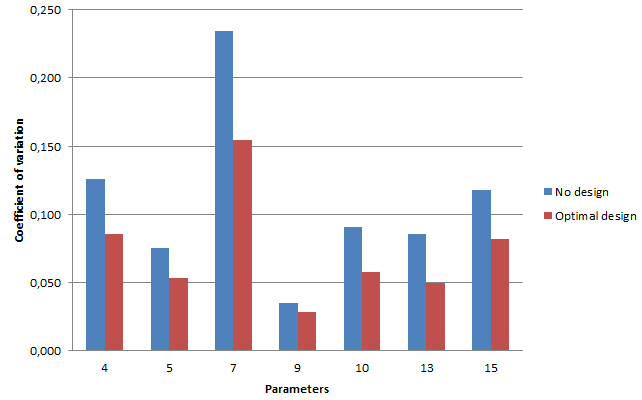
\epsfig{file=Figures/Bergmanoptdesign3days.png, width=\textwidth}\caption{A comparison of identifiability for each parameter with and without the experiment design for the case of a three meals monitoring.}
\label{fig:Bergmanoptdesign3days}
\end{figure}

A remarkable fall in the coefficient of variation is observed for all the parameters, and not just for the general identifiability of the model. In the original sensitivity analysis of Bergman's model all the parameters were selected to be identifiable, assuming identifiability of the model when all its parameters presented CVs below 30\%. For Bergman's model the limitant parameter (highest CV) was parameter 7, $K_{max}$. Using experiment design we reduce the variability of this parameter to half of the identifiability threshold, not sacrificing identifiability in any of the other parameters.

\section{Experiments designed with modified Panunzi's model}
\label{sec:ExperimentsDesignedWithPanunziSModelModified}

Identifiability of the modified version of Panunzi's endogenous model, which was described in Section \ref{sec:CriticalSelectionOfModels} will be analyzed next. Modified Panunzi's model and the two input models already used for Bergman's system comprise a total of 16 parameters, 4 of which correspond to the endogenous model. The 16 parameters are described in Table \ref{tab:panunziparameters}.

\begin{table}[hbt]
  \begin{center}
	\begin{tabular}{| c | c | c | c |}
	\hline 
	Model	& Number & Parameter & Meaning \\
	\hline 
	Endogenous & 1 & $K_{xgl}$ & Insulin sensitivity \\
	 & 2 & $V_{g}$ & Distribution volume of glucose\\
	 & 3 & $T_{gh}$ & Hepatic balance \\
	 & 4 & $k_{i}$ & Insulin action delay \\
	\hline
	Gastric & 5 & $K_{abs}$ & Glucose absorption rate in the gut \\
	 & 6 & $K_{max}$ & Maximum gastric emptying rate \\
	 & 7 & $K_{min}$ & Minimum gastric emptying rate \\	
	 & 8 & $b$ & Involved in the gastric emptying \\
	 & 9 & $c$ & Involved in the gastric emptying \\
	\hline
	Insulin & 10 & $V_{i}$ & Distribution volume of insulin \\
	 & 11 & $k$ & Proportion of insulin in the slow channel \\
	 & 12 & $k_{a1}$ & Transfer rate in the slow channel \\
	 & 13 & $k_{a2}$ & Transfer rate in the fast channel \\
	 & 14 & $k_{e}$ & Insulin elimination \\
	 & 15 & $V_{MAX,LD}$ & Michaelis-Menten parameter \\
	 & 16 & $k_{M,LD}$ & Michaelis-Menten parameter \\
	\hline	
	\end{tabular}
  \end{center}
  \caption{Parameters to be identified in Modified Panunzi's model.}
	\label{tab:panunziparameters}
\end{table}

Many of the parameters involved in the sensitivity analysis for Bergman's endogenous model are repeated for this case, but the numeration is different due to the different number of parameters in the endogenous model. The results of the identifiability study are shown in Table \ref{tab:panunziCV}.

\begin{table}[hbt]
	\centering
	\begin{tabular}{ c | c | c | c | c | c | c }
	\multirow{2}{*}{Number} & \multirow{2}{*}{Parameter} & \multicolumn{5}{c}{Iteration} \\
	& & 1 & 2 & 3 & 4 & 5 \\
	\hline 
	1 & $K_{xgl}$ & 1.14 & 0.98 & 0.55 & 0.53 & 0.31\\
	2 & $V_{g}$ & 0.46 & 0.43 & 0.26 & 0.24 & 0.23\\
	3 & $T_{gh}$ & 0.51 & 0.18 & 0.18 & 0.18 & 0.06\\
	4 & $k_{i}$ & 4.91 & - & - & - & -\\
	5 & $K_{abs}$ & 1.60 & 1.12 & 0.67 & - & -\\
	6 & $K_{max}$ & 0.78 & 0.66 & 0.53 & 0.24 & 0.24\\
	7 & $K_{min}$ & 0.87 & 0.68 & 0.33 & 0.33 & 0.30\\	
	8 & $b$ & 0.41 & 0.20 & 0.18 & 0.17 & 0.13\\
	9 & $c$ & 0.66 & 0.51 & 0.34 & 0.20 & 0.18\\
	10 & $V_i$ & - & - & - & - & -\\
	11 & $k$ & 0.91 & 0.81 & 0.36 & 0.29 & 0.27\\
	12 & $k_{a1}$ & 0.45 & 0.43 & 0.26 & 0.25 & 0.20\\
	13 & $k_{a2}$ & 3.77 & 2.57 & - & - & -\\
	14 & $k_{e}$ & 0.88 & 0.71 & 0.49 & 0.49 & 0.30\\
	15 & $V_{MAX,LD}$ & 1.92 & 0.92 & 0.66 & 0.62 & -\\
	16 & $k_{M,LD}$ & - & - & - & - & -\\	
	\end{tabular}
\caption{Modified Panunzi's model parameter coefficients of variation (CV) for a three meals identification.}
\label{tab:panunziCV}
\end{table}

Following the same methodology than in the Bergman's model analysis, only two parameters were not identifiable because of FIM singularity. These two parameters (10 and 16) show in Table \ref{tab:panunziCV} with their row in the first iteration blank. Parameter 16 is fixed in the identification because of its low sensitivity, and parameter 10 is fixed to its nominal value due to a very strong correlation (proportional relation) to parameter 1. Five iterations on the sensitivity analysis were needed for the modified Panunzi's model in order to obtain a feasible set of parameters for identification, to produce a 10 parameter set with good identifiability.

The set of parameters in the last column of Table \ref{tab:panunziCV} is considered the optimum set of parameters for identification even though 3 of the parameters of that set present CVs in the acceptable limit of identifiability (30\%). Those parameters ($K_{xgl}$, $K_{min}$ and $k_{e}$) in the proposed limit of identifiability are considered of great importance for the identification of individual patients in the postprandial period. $K_{xgl}$ represents the insulin sensitivity of the patient, a parameter that is known to present high inter and intra-patient variability, thus needed to be subject to identification. $K_{min}$ stands for one of the parameters defining gastric emptying, also very variable between and within patients. $k_{e}$ is the insulin elimination rate, and strongly affects the insulin dynamics and overall sensitivity of the patient. All these parameters were sensitive to identification in diabetic patients, and were decided to be included in the optimal set, following the proposed methodology. The summary of identifiable parameters is explained in Figure \ref{fig:panunziparametersidentifiable}.

\begin{figure}[hbtp]
\centering
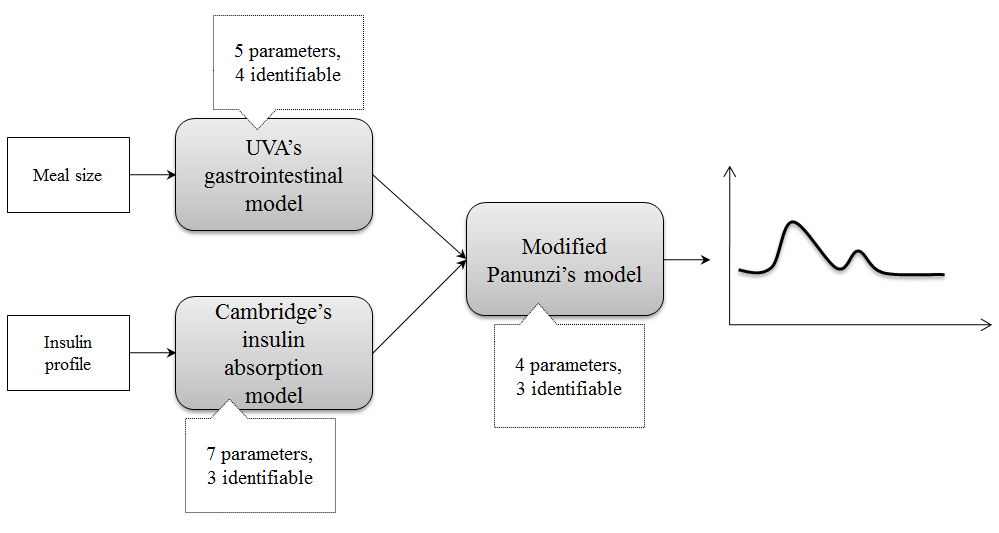
\epsfig{file=Figures/panunziparametersidentifiable.png, width=\textwidth}\caption{Optimal set of parameters for the modified Panunzi's model combined with UVA's gastrointestinal model and Cambridge insulin absorption.}
\label{fig:panunziparametersidentifiable}
\end{figure}

These 10 parameters will be used in the experiment design for the calculation of the index of total identifiability of the model. All identifiable parameters are distributed amongst all the submodels of the modified Panunzi's system. The same approach of multiple day identifications used for the optimal experiment design of Bergman's model is used in here. In the next lines, experiments designed comprising one, two, three and four days of monitoring are displayed.

\begin{itemize}
\item{The results of an experiment designed for \textit{one} day of monitoring consisting on the five following hours to a meal are: $\tau = -17.95$ minutes, Meal $= 100$ g CHO and Bolus $=10$ IU. The same profile as in the Bergman's model experiment design is observed in the modified Panunzi's experiment for the one-day monitoring. The insulin bolus is not as advanced as in Bergman's model design, but the meal and bolus size are again in the maximum value of the constrained optimization. Separation of dynamics of the insulin absorption system is the best option for the one-day monitoring scenario. The response of the new model to the experiment designed is shown in Figure \ref{fig:optdesignpanunzi1day}.

\begin{figure}[hbt]
\centering
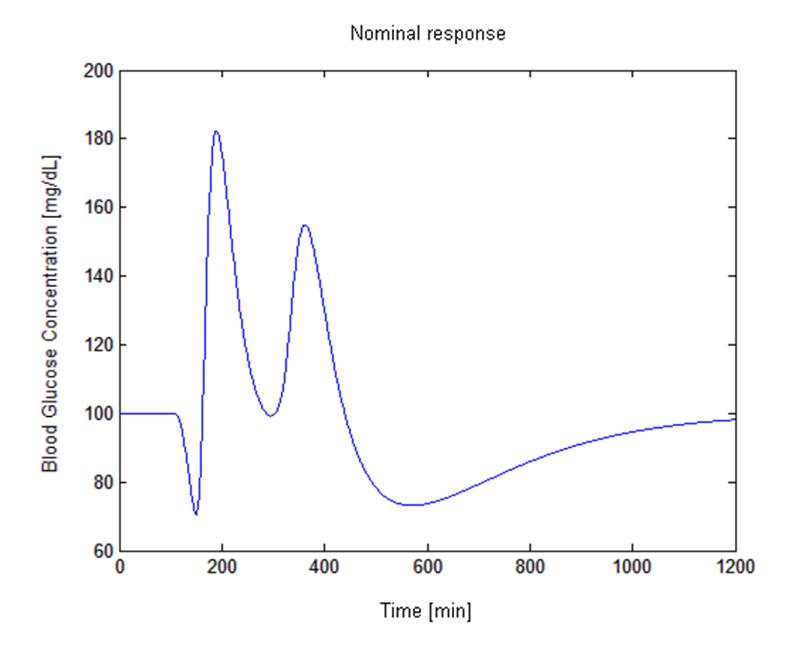
\epsfig{file=Figures/optdesignpanunzi1day.png, width=0.9\textwidth}\caption{Modified Panunzi's model response to the proposed experiment for 1 day. Meal is ingested at time 120 min.}
\label{fig:optdesignpanunzi1day}
\end{figure}

Comparing modified Panunzi's model response in a single day experiment with the Bergman's model response (Figure \ref{fig:bergmanexperiment1day}), the glucose profile is virtually identical. This fact may lead to two conclusions: 1) Using simple endogenous models, the dynamics of the input models direct the behavior of glucose concentration; 2) the optimization of identifiability is not strongly dependent on the endogenous models used. Indeed the model's parameters are different in each model, but the signal from where information is being extracted is the same, and regarding that signal from a theoretical point of view, the optimal glucose profile in terms of containing information, must be very rich in information for any other model too. That is why it is expected of optimal experiment glucose outcomes to be similar for the modified Panunzi's model to the results for the other experiments already designed.}

\item{The conditions of experiment designed \textit{two} day monitoring are:

\begin{itemize}
	\item Day 1. $\tau = 157.80$ minutes, Meal $= 44.25$ g CHO and Bolus $=3.07$ Insulin Units
	\item Day 2. $\tau = -17.92$ minutes, Meal $= 100$ g CHO and Bolus $=9.99$ Insulin Units
\end{itemize}

The second day in this experiment is the same as the single day experiment, in which the bolus is administered in advance to the meal time, thus only the insulin system is being excited in that period. In the first day, a new situation is proposed, similar to the case of Bergman's design in which the bolus was delayed, but in this case, the delay is much bigger. However, delaying the insulin bolus up to two hours and a half can be quite dangerous for the patient because of risks of hyperglycemia, that is why the meal size is much smaller for this large delay case, in order to keep the glucose profile within safety constraints. In Figure \ref{fig:optdesignpanunzi2day} the response of the model to the experiment proposed can be observed.

\begin{figure}[hbt]
\centering
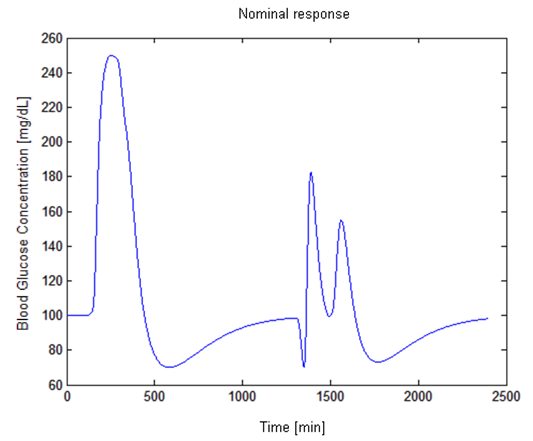
\epsfig{file=Figures/optdesignpanunzi2day.png, width=0.9\textwidth}\caption{Modified Panunzi's model response to the proposed experiment for a 2 days monitoring. Meals are ingested at time 120 and 1020 min.}
\label{fig:optdesignpanunzi2day}
\end{figure}

In the case of the first day  the small amount of carbohydrates given to the patient (44.25 grams) has the objective of rising the blood glucose up to the superior limit of safety of the patient. The insulin bolus is given when the blood glucose gets to the maximum established, and the amount of insulin given is so that it will force the blood glucose down to the lower safety constraint. Again, the experiment design is exciting the glucose signal used for identification from one boundary to the other, in order to maximize the amount of information contained in the glucose signal. Bergman's model was probably not able rise so fast up to the limit of hyperglycemia due to the so called term of glucose efficiency (as explained in Section \ref{sec:CriticalSelectionOfModels}) that makes glucose to drop automatically when it rises above the stability point. As this term is not present in the modified Panunzi's model, glucose dynamics are much faster and permit stronger excitations from the inputs, which is more realistic.}

\item{The conditions of experiment designed \textit{three} day monitoring are:
\begin{itemize}
	\item Day 1. $\tau = -17.83$ minutes, Meal $= 100$ g CHO and Bolus $=10$ Insulin Units
	\item Day 2. $\tau = -18.42$ minutes, Meal $= 100$ g CHO and Bolus $=10$ Insulin Units
	\item Day 3. $\tau = 165.74$ minutes, Meal $= 44.38$ g CHO and Bolus $=3.01$ Insulin Units
\end{itemize}


In this case the advanced bolus administration is given in two out of the three days of the experiment, while the other day a small meal is given, with the insulin bolus delayed 165 minutes, just like in the two days experiment. The fact that the ``bolus given in advance'' scenario is repeated proves that there is more information to be extracted from the excitation of the insulin absorption model than in the rest of the system. This conclusion is repeated for both model's experiment design. The simulated glucose profile of the model is shown in Figure \ref{fig:optdesignpanunzi3day}.

\begin{figure}[hbt]
\centering
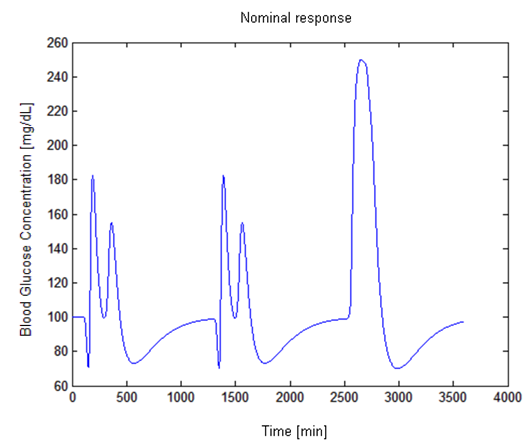
\epsfig{file=Figures/optdesignpanunzi3day.png, width=0.9\textwidth}\caption{Modified Panunzi's model response to the proposed experiment for a 3 days monitoring. Meals are ingested at time 120, 1020 and 1920 min.}
\label{fig:optdesignpanunzi3day}
\end{figure}


This is a very good example of how the different experiments designed for each independent day are not dependent on the order of those days. Sometimes the case of the small meal and delayed bolus happens in the first day, some others at the end, and it can also be in the middle of the 3 days. Also, it is confirmed that increasing the number of experiments causes the richest information postprandial period to repeat in order to maximize the identifiability. No further synergies between different days where observed, and every day is independent in the optimization algorithm.}

\item{The conditions of experiment designed for the final case of \textit{four} day monitoring are:
\begin{itemize}
	\item Day 1. $\tau = 167.06$ minutes, Meal $= 44.25$ g CHO and Bolus $=3$ Insulin Units
	\item Day 2. $\tau = -17.22$ minutes, Meal $= 100$ g CHO and Bolus $=10$ Insulin Units
	\item Day 3. $\tau = -18.41$ minutes, Meal $= 100$ g CHO and Bolus $=10$ Insulin Units
  \item Day 4. $\tau = 86.19$ minutes, Meal $= 47.07$ g CHO and Bolus $=4.13$ Insulin Units
\end{itemize}

The conditions for day four are a little bit different than the previous ones, but it hardly defines a new type of therapy for a day of identification. It is a variation of the profile with a small meal and delayed insulin bolus shown in day one, considering a smaller delay so that the insulin bolus has not only a role of correction of the level of blood glucose, but also tries to counteract the rise of blood glucose that is still coming from the gut. That is observed in Figure \ref{fig:optdesignpanunzi4day}, where the time of administration of the bolus does not wait for the blood glucose to stop rising and get stabilized, and instead, it forces it down before the absorption is over.}
\end{itemize}

\begin{figure}[hbt]
\centering
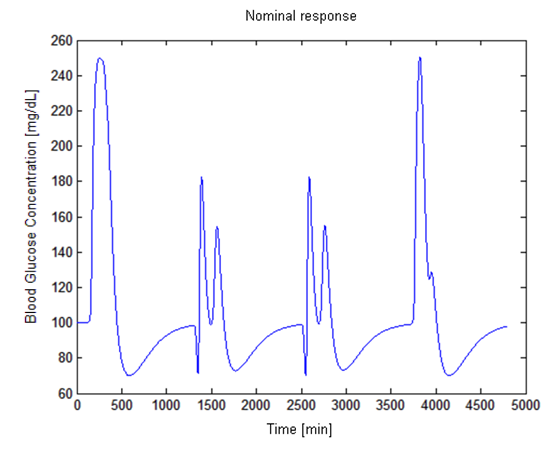
\epsfig{file=Figures/optdesignpanunzi4day.png, width=0.9\textwidth}\caption{Modified Panunzi's model response to the proposed experiment for a 4 days monitoring period. Meals are ingested at time 120, 1020, 1920 and 2820 min.}
\label{fig:optdesignpanunzi4day}
\end{figure}

As a summary, with the optimal set of parameters of the modified Panunzi's model, two different profiles of glucose are determinant for the good identification of the model.
\begin{itemize}
	\item The first therapy has already been seen in Bergman's model experiment design, and it consists of an advance of the bolus of insulin to the meal time, improving the identifiability of the insulin subsystem.
	\item The second therapy consists on a big delay (2-3 hours) in the administration of the bolus, while giving a small amount of carbohydrates (40-50 grams) to avoid severe hyperglycemia. With this therapy, separation of insulin and glucose dynamic from the meal is obtained, while maintaining plasma glucose in a safe range.
\end{itemize}

In Figure \ref{fig:panunzidays} the evolution with the number of days of the parameters identifiability is shown for the optimal set of parameters.

\begin{figure}[hbtp]
\centering
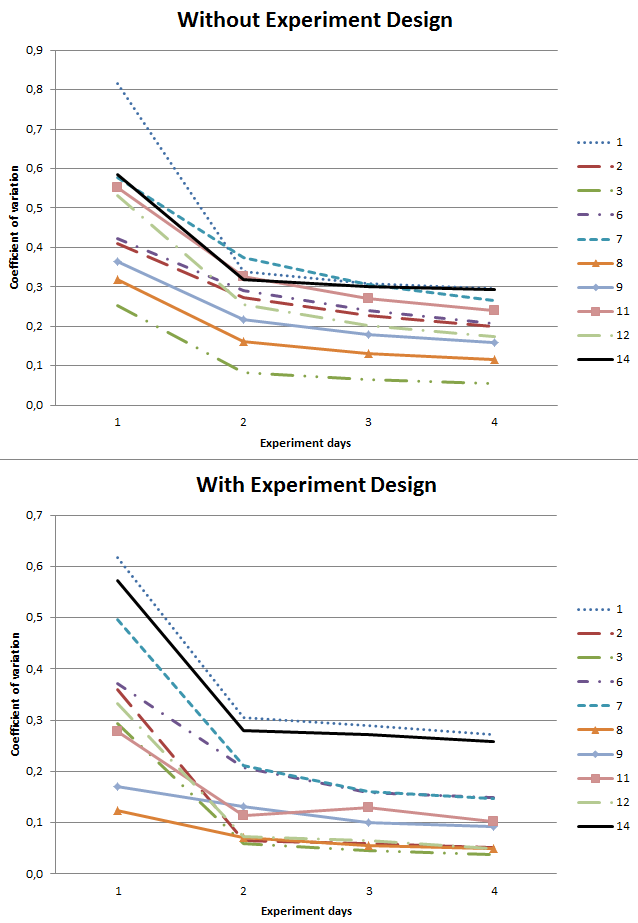
\epsfig{file=Figures/panunzidays.png, width=0.8\textwidth}\caption{Modified Panunzi's optimal set of parameters and their coefficients of variation as they get smaller with the number of monitoring days. Top graph shows the evolution of the parameters' identifiability with experiment length. Bottom panel displays the identifiability of the same parameters applying the designed experiments.}
\label{fig:panunzidays}
\end{figure}

The graphs are very similar to those seen in the analysis of Bergman's model. The influence of the number of days, especially between days one and two, is very important both in the case of experiment and no experiment design. It is worth noting the difference on scale between the top and bottom panel. While without experiment design the parameter's CVs start in some cases as high as 0.8, applying optimization of identifiability this starting variability is reduced to approximately 0.6. Again, a minimum of two days is required for optimal identifiability of the whole system, because of the great drop of CVs of all the parameters in the system, but also because of the inclusion of both therapies proposed which guarantee the separation of dynamics of both input systems. For the same reasons exposed in Bergman's model analysis, a three days experiment is preferred, and it concurs with the findings of the experiment design using modified Panunzi's model.

The influence of the experiment design in the identifiability of the model can clearly be seen in Figure \ref{fig:panunzi1optdesign3days}, where it is shown that experiment design improves identifiability dramatically. In this case, identifiability of almost all the parameters rises, getting their coefficients of variation divided by two or three. Special cases are the parameters 1 and 14, whose identifiability rises to a smaller extent. This resistance to change in the identifiability might be explained by the strong correlation between these two parameters since both of them are very related to the plasma insulin dynamics and its influence in blood glucose (parameter 1, $K_{xgl}$, is the insulin sensitivity and parameter 14, $k_{e}$, is the plasma insulin elimination). On the contrary, $V_g$ identification improves dramatically with experiment design.

\begin{figure}[hbt]
\centering
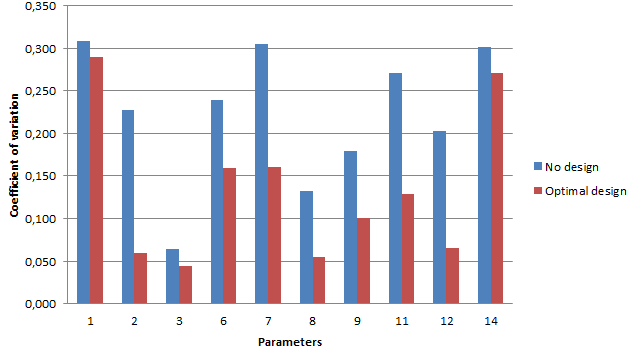
\epsfig{file=Figures/panunzi1optdesign3days.png, width=\textwidth}\caption{Identifiability of the optimal set of parameters of modified Panunzi's model before and after the experiment design for the case of a three meals monitoring.}
\label{fig:panunzi1optdesign3days}
\end{figure}

\section{Discussion and clinical protocol}
\label{sec:DiscussionAndProtocol}

Identifiability has been drastically improved in both models, but in theory, the experimental design should not end here. The optimal design requires of interaction with the experimental setup in order to keep improving the conditions of the identification. For example, the assumption of nominal values in the parameters for the analysis and experiment design may be questionable, and every identification performed on real data must be subject to an identifiability analysis. With the collection of new experimental data, we may be able to design further experiments based on a new nominal value on the parameter space.

Up to this point, only two models were tested following the exposed methodology, but the experiment design is open for more models to be challenged in their identifiability. When looking at the identifiability analysis, it was accepted that a parameter was identifiable if its CV was below 0.3. After the optimal experiment design, the optimal set of parameters has had the CVs of all its parameters reduced in many cases far below the 0.3 threshold. Naturally, the question arises: ``what if more parameters were included in the \textit{optimal} set?''. `It is very much possible that those parameters CV drop below the identifiability threshold after the optimization of identifiability. However, it is impossible to know this \textit{a priori}, and a iterative approach must be used to check this hypothesis. Unfortunately, optimal experiment design is a very heavy computation task, and embedding it in an iterative paradigm seems unreasonable, and thus this hypothesis is discarded.

The results of the experiment design do not have to be taken literally in practice. The assumptions made when using each model with its nominal parameters have great importance on the results of the experiment design. From a practical point of view, experimenting with several different models allows us to draw some general qualitative conclusions. That is why the design has been repeated several times in this thesis. Qualitative and common characteristics of the experiments designed are extracted in the next lines, trying to get the most important features needed in a monitoring for the good posterior identification of a patient, regardless of the model used.

The experiment design aims to separate the dynamics of the sub-models for a better identification. There are two different single day experiments present: in one case insulin dose is given without meal perturbation, limited by the hypoglycemia constraint, in order to obtain information of the subcutaneous insulin model. The other situation is exactly the opposite: a meal is given while the insulin dose is delayed limited by the hyperglycemia constraint. During this time, the intestinal absorption model is the only one acting on the output signal. Optimal experiment design forces the model to move in all the range of operation set in order to preserve patient's safety, thus extracting more information out of the data. Maximum excitation of the model is required, while separating the perturbations to the output signal for maximum identifiability.

The application of the designed experiment in ambulatory conditions is not straightforward. In the optimal experiment design the (virtual) patient is supposed to be stabilized into euglycemic range. In real experiments, even during the fasting state, patients may not be under steady state conditions, presenting glucose concentration measurements in any glycaemic range. Under these circumstances, application of the optimal experiment design to the clinical setting requires some cautions. Indeed, if the patient is hyperglycemic at the beginning of the experiment, delaying more than two hours the insulin dose can be dangerous for the patient's health, with extremely high glucose values. On the other hand, if the patient is hypoglycemic (or prone to hypoglycemia) in the preprandial period, administrating an insulin dose without carbohydrates ingestion can lead to severe hypoglycemia. 

Therefore, an adaptation of the optimal experiment design to the initial metabolic state of the patient is proposed \cite{DTMlaguna2010}. For every major meal of the day, if the patient starts the monitoring with a blood glucose level over 150 mg/dL or in the 100-150 mg/dL range with an increasing trend (hyperglycemic risk), the insulin bolus is given followed 30 minutes later by a 100 grams meal. If the glucose level is below 100 mg/dL or in the 100-150 mg/dL range with a decreasing trend (hypoglycemic risk), a 40 or 60 (patient's choice) grams meal is given and the insulin dose administration is delayed 120 minutes. In both situations the dose to be administered is the one recommended to the patient, depending on the size of the meal and his/her usual insulin-to-carbohydrate ratio. The patient can choose among three menus with the same relative nutritional composition. With this protocol the separation of dynamics is achieved, while minimizing risks for the patients. This protocol is summarized in table \ref{tab:protocol}.

\begin{table}[hbt]
	\centering
	\begin{tabular}{| p{0.4\textwidth} | p{0.5\textwidth} |}
	\hline 
	\textbf{Pre-prandial glycemia} & \textbf{Action}\\
	\hline 
	Greater than $150 mg/dL$ or between $100-150$ and rising & Infusion of an insulin bolus 30 minutes before of 100 grams meal \\
	\hline 
	Lower than $100 mg/dL$ or between $100-150$ and decreasing & 40 grams meal and bolus infusion 2 hours later \\
	\hline 
	\end{tabular}
\caption{Clinical protocol for application on ambulatory experiments.}
\label{tab:protocol}
\end{table}

The protocol was approved by the Ethical Committee of the Clinic University Hospital of Valencia and home-made monitoring was performed for validation of the identification procedure. Patients were monitored during two weeks, with a wash-up week in between, and instructed to follow the protocol defined by the experiment design. Twelve subjects with T1DM under long-term intensive insulin treatment with CSII (nine women; 41.8 - 7.3 years old; diabetes' duration, 20.2 - 10.3 years; body mass index, 25.1 - 2.8 $kg/m^2$; glycosylated hemoglobin [A1C], 8.0 - 0.6\%; basal insulin dose, 0.8 - 0.3 U/h; I:CHO ratio, 1.3 - 0.5 U/10 g of CHO [mean - SD]) were studied in the hospital (inpatient study) following a period of ambulatory CGM. In the ambulatory period the subjects underwent at least two outpatient 6-day periods of CGM monitoring for the identification (the first 3 days) and validation (the last 3 days) of an individualized model to be used in the prediction of the 5-h postprandial period. In order to account for intra-patient variability, a prediction model with interval parameters was calculated from the previous identified model considering 20\% uncertainty in insulin sensitivity and 10\% in CHO estimation. The interval model was validated during the last 3 days of CGM, where the patients had a standardized meal daily (40-g, 60-g, or 100-g CHO content, depending on the pre-prandial glucose readings). Unfortunately, validation had to be performed over CGM readings, leading to non-conclusive results. Glucose gold reference data are required for the successful validation of an identification study on diabetic patients, since noisy measurements in the validation days can affect the results of the validation, and therefore the overall performance of the identification experiment.

The data acquired using this protocol was later used to test new computer generated insulin treatments for diabetic patients \cite{paoloibolus2012}. Pilot identifications were performed on the domiciliary data, and the identified models were used for the computation of adjusted-to-patient insulin therapies in a full randomized double-blind study. Although the identification performance was not excellent, they yielded reasonable insulin therapies to be used in clinic that were approved by the medical committee. The main limitation of the identifications performed was that no uncertainty was considered in the identification. Uncertainty was artificially added for the validation, and it was considered to be the same for every patient, which lead to incomplete characterization of the patient. In further experiments, uncertainty must be included in the identification methods.

On the clinical part of the experiments performed, subjects were admitted to the Endocrine Clinical Research Center of the Clinic University Hospital of Valencia, Valencia, Spain, at 09:00 h. They were put in the sitting position, and two venous lines were prepared: one for arterialized venous blood sampling and the other for insulin or glucose infusion, if required. Indeed, to ensure comparable metabolic conditions between studies, where appropriate, subjects received an intravenous infusion of regular human insulin following a feedback procedure to maintain PG close to 90 mg/dL until the beginning of the studies at 13:00 h (time 0 of the study). Then, the test mixed-meal was consumed in 15-20 min. At the same time, insulin was administered following the randomization schedule, and PG was monitored for 5 h, until the end of study at 18:00h (time 300 min). In order to avoid hypoglycemia during time 0-300 min, a controlled glucose infusion was started if blood glucose fell below 75 mg/dL, and the pre-meal glycaemic levels were maintained (euglycemic clamp). 

Similar results were observed in the in-hospital part of the experiment for the regular insulin treatment, which is adjusted by medical experts, and the computer generated insulin therapy. This findings lead to the conclusion that CGM-based algorithm for the calculation of prandial insulin is feasible, although it does not reduce unpredictability of individual glycaemic responses.



